\documentclass{beamer}
\usetheme{Madrid}

\AtBeginSection[]{
  \begin{frame}
  \vfill
  \centering
  \begin{beamercolorbox}[sep=8pt,center,shadow=true,rounded=true]{title}
    \usebeamerfont{title}\insertsectionhead\par%
  \end{beamercolorbox}
  \vfill
  \end{frame}
}

\makeatletter
\setbeamertemplate{footline}{%
  \leavevmode%
  \hbox{%
  \begin{beamercolorbox}[wd=.2\paperwidth,ht=2.25ex,dp=1ex,center]{author in head/foot}%
    \usebeamerfont{author in head/foot}\insertshortauthor\expandafter\beamer@ifempty\expandafter{\beamer@shortinstitute}{}{~~(\insertshortinstitute)}
  \end{beamercolorbox}%
  \begin{beamercolorbox}[wd=.6\paperwidth,ht=2.25ex,dp=1ex,center]{title in head/foot}%
    \usebeamerfont{title in head/foot}\insertshorttitle
  \end{beamercolorbox}%
  \begin{beamercolorbox}[wd=.2\paperwidth,ht=2.25ex,dp=1ex,right]{date in head/foot}%
    \usebeamerfont{date in head/foot}\insertshortdate{}\hspace*{2em}
    \insertframenumber{} / \inserttotalframenumber\hspace*{2ex} 
  \end{beamercolorbox}}%
  \vskip0pt%
}
\makeatother


%Packages
\usepackage[utf8]{inputenc}
\usepackage{hyperref}
\usepackage{amssymb}

%META-INFORMATION
\title[Semantic Documents and Dynamic Notebooks]{Integrating Semantic Mathematical Documents and Dynamic Notebooks}
\author[Tom Wiesing et al.]{Kai Amann, Michael Kohlhase, Florian Rabe, and \underline{Tom Wiesing}\\Computer Science, FAU Erlangen-N{\"u}rnberg}
\date[July 12 2019, CICM Prague]{July 12, 2019\\Conference on Intelligent Computer Mathematic\\Prague, Czech Republic}

\begin{document}
    %TITLEPAGE
    \frame{\titlepage}

    %OVERVIEW
    \begin{frame}{Overview}
        \begin{itemize}
            \item Introduction
            \item A REPL to build mathematical documents
            \item Widgets for active documents
            \item Conclusion
        \end{itemize}
    \end{frame}

    \section{Introduction}

    \begin{frame}{Introduction -- Documents}
        \begin{columns}
        \column{0.7\textwidth}
            \begin{itemize}
                \item \textbf{Documents} guide the user through a particular topic
                \begin{itemize}
                    \item Papers
                    \item Talks
                    \item Books
                    \item Websites
                \end{itemize}
                \item Useful for \textbf{communicating} knowledge
                \item Caveat: Documents are usually \textbf{static}
                \begin{itemize}
                    \item they do not allow interaction with this knowledge
                \end{itemize}
                \item Focus on \textbf{Mathematical Documents} in this talk
                \begin{itemize}
                    \item can be generalized to all of \textbf{STEM}
                \end{itemize}
            \end{itemize}
                \column{0.3\textwidth}
            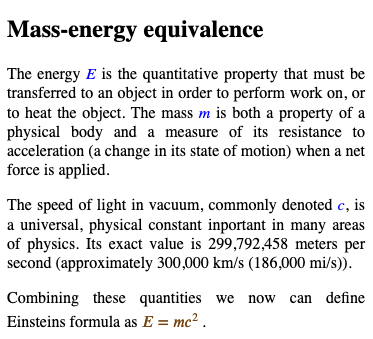
\includegraphics[scale=0.25]{images/doc}
        \end{columns}
    \end{frame}

    \begin{frame}{Introduction -- What is a REPL?}
        \begin{columns}
        \column{0.5\textwidth}
            \begin{itemize}
                \item REPL = \textbf{R}ead \textbf{E}val \textbf{P}rint \textbf{L}oop
                \begin{enumerate}
                    \item\label{replbegin} Read a Command from the user
                    \item Evaluate the Command
                    \item Print the Result
                    \item Loop back to \ref{replbegin}
                \end{enumerate}
                \item commonly used for programming or command line interaction
                \begin{itemize}
                    \item e.g. Bash (Linux / Mac OS) or PowerShell (Windows)
                    \item e.g. Python (scientific programming)
                \end{itemize}
            \end{itemize}
        \column{0.5\textwidth}
            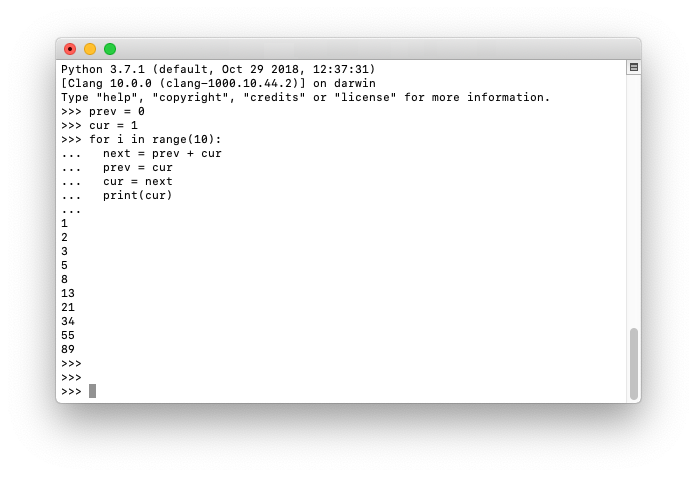
\includegraphics[scale=0.25]{images/repl}
        \end{columns}
    \end{frame}

    \begin{frame}{Notebooks}
        \begin{columns}
        \column{0.5\textwidth}
            \begin{itemize}
                \item REPL = \textbf{R}ead \textbf{E}val \textbf{P}rint \textbf{L}oop
                \begin{enumerate}
                    \item\label{replbegin} Read a Command from the user
                    \item Evaluate the Command
                    \item Print the Result
                    \item Loop back to \ref{replbegin}
                \end{enumerate}
                \item commonly used for programming or command line interaction
                \begin{itemize}
                    \item e.g. Bash (Linux / Mac OS) or PowerShell (Windows)
                    \item e.g. Python (scientific programming)
                \end{itemize}
            \end{itemize}
        \column{0.5\textwidth}
            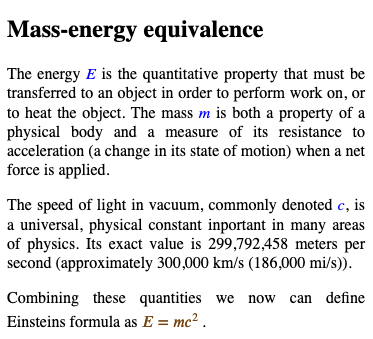
\includegraphics[scale=0.25]{images/doc}
        \end{columns}
    \end{frame}

\end{document}